\documentclass[svgnames,11pt]{beamer}
\input{/home/tof/Documents/Cozy/latex-include/preambule_commun.tex}
\input{/home/tof/Documents/Cozy/latex-include/preambule_beamer.tex}
%\usepackage{pgfpages} \setbeameroption{show notes on second screen=left}
\author[]{Christophe Viroulaud}
\title{Gestion d'une collection de bandes-dessinées\\Modèle relationnel}
\date{\framebox{\textbf{BDD 01}}}
%\logo{}
\institute{Terminale - NSI}

\begin{document}
\begin{frame}
\titlepage
\end{frame}
\begin{frame}
    \frametitle{}

    Pour gérer son importante collection de bandes-dessinées, les nouveautés mais également les emprunts, le professeur veut s'appuyer sur un modèle informatique.
    \begin{center}
    \centering
    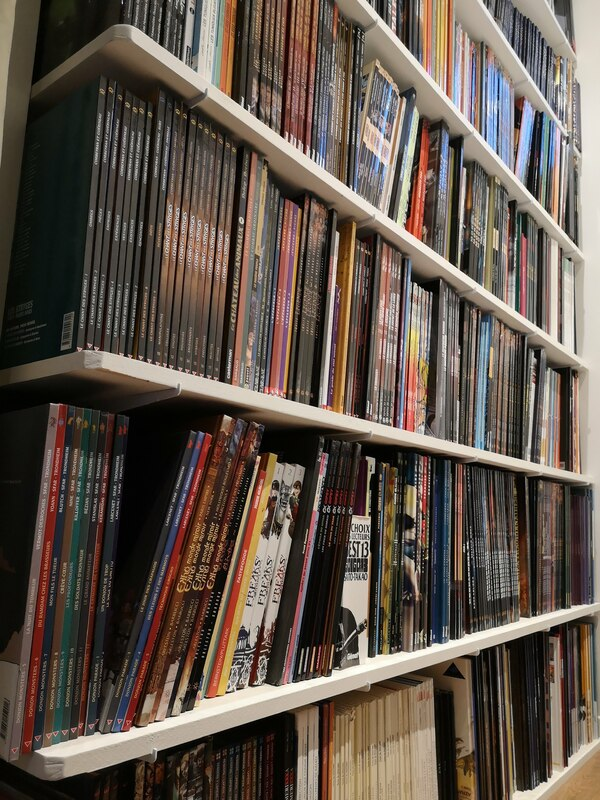
\includegraphics[width=4.5cm]{ressources/biblio.jpg}
    \captionof{figure}{Extrait de la collection}
    \label{IMG}
    \end{center}

\end{frame}
\begin{frame}
    \frametitle{}

    \begin{framed}
        Quelle solution mettre en place pour gérer efficacement une grande quantité de données?
    \end{framed}

\end{frame}
\section{Solution naïve: le tableur}
\begin{frame}
    \frametitle{Solution naïve: le tableur}

    \begin{center}
    \centering
    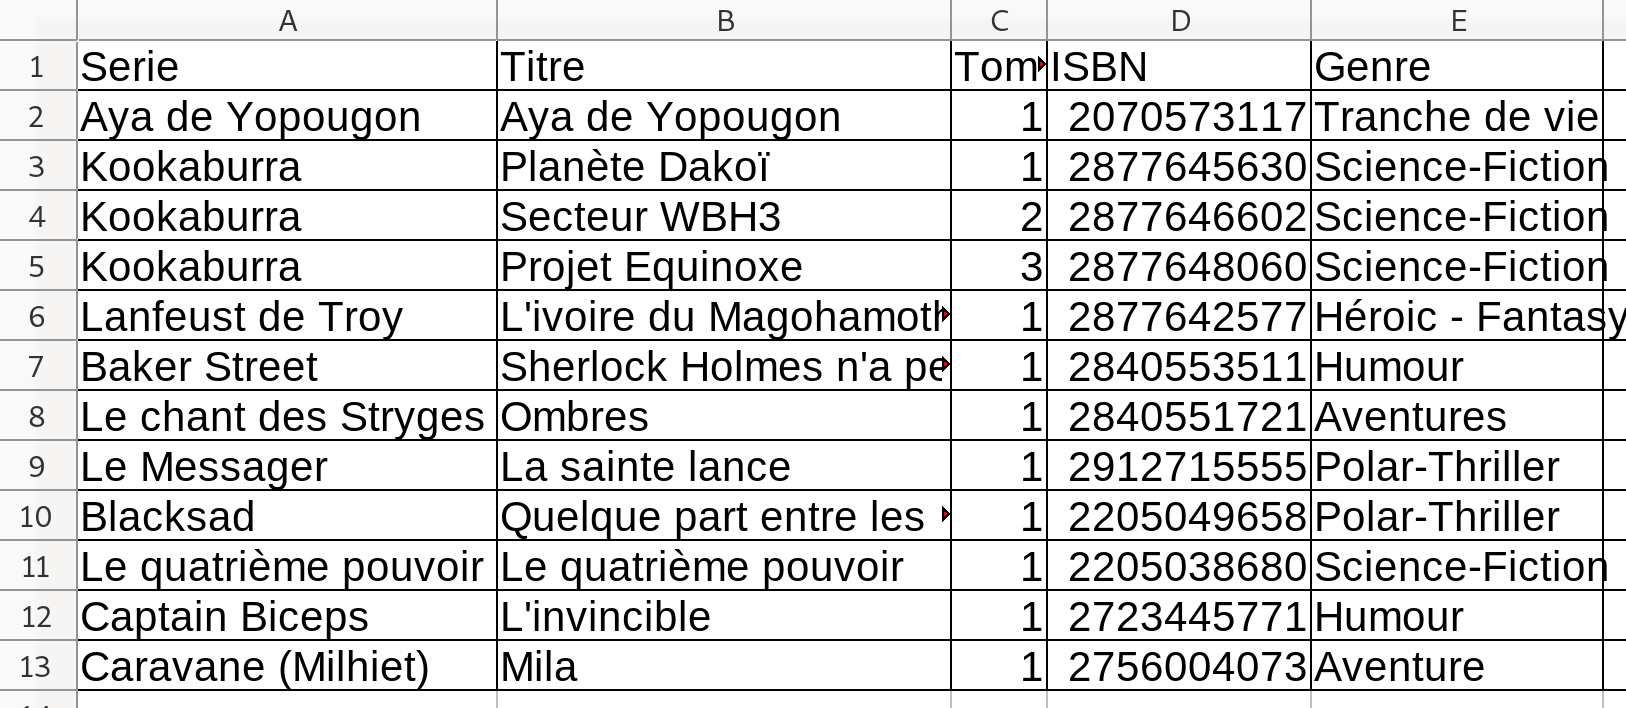
\includegraphics[width=10cm]{ressources/approche-1.png}
    \captionof{figure}{Utilisation d'un fichier \textbf{\texttt{CSV}}}
    \label{IMG}
    \end{center}
\begin{activite}
    Établir les limites de cette approche.
\end{activite}
\end{frame}
\begin{frame}
    \frametitle{Correction}

    \begin{itemize}
        \item Gestion de grandes quantités de données?
        \item Gestion des modifications efficacement (ex: changement titre d'une série)?
        \item Gestion des informations \emph{externes} (ex: informations sur les emprunteurs)?
    \end{itemize}
\note[item]{Python peut gérer un csv de 2000 lignes, mais si s'agrandit?}
\note[item]{pb tableur $\;\rightarrow\;$ article "malades du covid oubliés"}
\note[item]{Si on veut + d'infos sur emprunteurs: nouvelles colonnes? ais une modif = beaucoup de changement}
\end{frame}
\section{Modèle relationnel}
\begin{frame}
    \frametitle{Modèle relationnel}

    

\end{frame}
\end{document}